\documentclass[12pt]{article}

\usepackage[english]{babel}                          
\usepackage[utf8]{inputenc}                                                           
\usepackage[math]{iwona}
\usepackage[T1]{fontenc}                         
\usepackage[margin=1.5cm, vmargin=1.5cm]{geometry}   
\usepackage{eurosym}
\usepackage{amsmath}
\usepackage{amssymb}
\usepackage{graphicx}
\usepackage{amsfonts}
\usepackage{multicol}
\usepackage{caption}
\usepackage{booktabs}
\usepackage{svg}
\usepackage{bm}

\author{Your name}
\title{Your title
}
\begin{document}
\makeatletter 
	\begin{titlepage} 
	\centering 
		{\large \textsc{Name of your laboratory}}\\ 
		\textsc{Name of your Matser's program}\\ 
	\vspace{1cm} 
		\includegraphics[width=\textwidth]{logo_cpht.png} \\
	\vspace{1cm} 
		{\large\textbf{	\@date\\
		 Internship Report}}\\ 
	\vfill 
		{\huge \textbf{\@title}} \\  \vspace{0.5cm}
		\LARGE subtitle \\
	\vspace{2em} 
		{\large \@author} \\ 
	\vfill 
		{\large Supervisor : } \\
	\end{titlepage} 
\makeatother

\tableofcontents

\section{Introduction}
\begin{multicols}{2}
Among layered materials, high-Tc superconductors, and especially cuprates, 
raised a lot of interest. Despite the numerous studies carried out on cuprates, 
the physics behind these compounds is not yet fully understood. The breakdown of 
BCS theory calls for more refined theories for explaining the unconventional 
superconductivity emerging \cite{Scalapino-rev}. Indeed, undoped cuprates turn 
out to be anti-ferromagnetic insulators \cite{damscelli-cuprates-review}, so no 
quasi-particle feature appears in their electronic structures preventing from 
the formation of coherent pairs, but the anti-ferromagnetic fluctuations do play 
an important role in the emergence of superconductivity with doping. 
Superconductivity is observed in hole-doped cuprates, suggesting that the 
question of superconductivity in cuprates is actually rather about how 
quasi-particles appear with doping. Once the quasi-particles appear, they are 
very much expected to form coherent pairs. This reasoning, along with the 
discovery of a rich phase diagram in respect of doping and temperature pushed 
the investigation of the underlying normal state of cuprates. \par The phase 
diagram for $\mathrm{Nd_{2-x}Ce_{x}CuO_{4}}$ and 
$\mathrm{La_{2-x}Sr_{x}CuO_{4}}$ \cite{damscelli-cuprates-review} is given in 
Fig. \ref{cuprate_phase_diag}. These two compounds are cuprates, whose phase 
diagram in general is close to those of other cuprates. In the undoped region, 
the cuprate is in an anti-ferromagnetic Mott insulator phase. With increasing 
hole doping (right part of the diagram) at zero temperature, the cuprate becomes 
superconducting, and at high doping it becomes a metal.
\begin{center}
    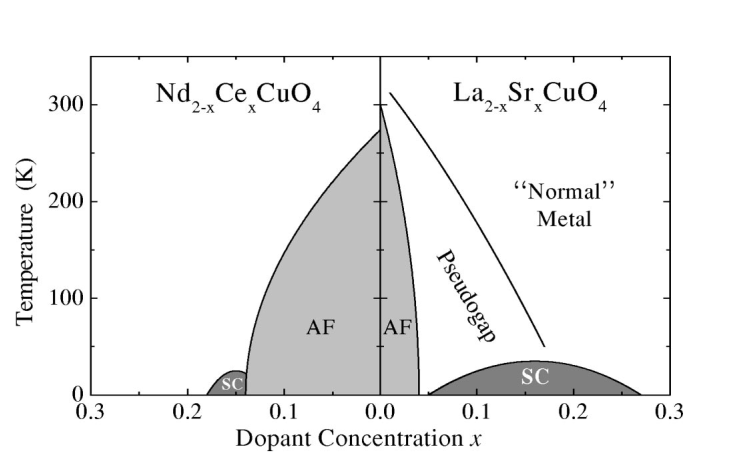
\includegraphics[width=\linewidth]{cuprates-PhaseDiag.png}
    \captionof{figure}{Phase diagram in respect of temperature and doping for $\mathrm{Nd_{2-x}Ce_{x}CuO_{4}}$ and $\mathrm{La_{2-x}Sr_{x}CuO_{4}}$. Taken from \cite{damscelli-cuprates-review}. Underdoped is said for a doping between zero and optimal doping, and overdoped is used for doping higher than optimal doping (see text).}
    \label{cuprate_phase_diag}
\end{center}
However, at higher temperatures for hole doping between x = 0.05 and x = 0.15 
the cuprate enters in the so-called pseudo-gap (PG) phase. The PG phase is 
characterized by the opening of an anisotropic gap (also called pseudo-gap) in 
the Brillouin zone at the Fermi energy \cite{alloul-PGdiscovery}. The pseudo-gap 
is robust as it remains even for temperatures far above the critical temperature 
for superconductivity ($T_{C}$), and it has similarities with the 
superconducting gap \cite{Ronning-CCOCARPES}. At temperatures close to the 
critical temperature for superconductivity, and for a doping close to the 
optimal doping (doping at which $T_{C}$ of superconductivity is the highest), 
the behavior of the critical line for the PG phase is still under debate. \par 
The similarities between the PG and the superconducting gap point out the fact 
that they could share the same origin, hence the study of the pseudo-gap seems 
crucial for the understanding of the cuprates' superconductivity. Our work takes 
place in this context : we aim at theoretically investigating the pseudo-gap 
phase in a specific cuprate $\mathrm{Ca_{2}CuO_{2}Cl_{2}}$ (CCOC). The choice of 
this compound was motivated by the fact that it has convenient surface 
properties for experiments\cite{Ronning-CCOCARPES} (which makes easier the 
comparison with theoretical results), and also because we will work along with 
researchers in Grenoble that can synthesize and analyze such compounds. The 
usual experiment for probing the pseudo-gap phase is Angle Resolved 
Photoemission Spectroscopy (ARPES) \cite{damscelli-cuprates-review}, but we will 
mainly focus here on the optical properties (optical conductivity for instance) 
of CCOC which can be used to highlight the emergence of a pseudo-gap. \par CCOC 
belongs to the class of layered materials, it consists of layers of 
$\mathrm{CuO_{2}}$ separated by Ca and Cl atoms in a tetragonal structure, see 
Fig. \ref{CCOC-struct}. Cu, O and Cl atoms form octahedras. The 
$\mathrm{CuO_{2}}$ layers are well separated hence they have a strong 2D 
character which is one of the essential aspects of high-$\mathrm{T_{C}}$ 
superconductors. Undoped CCOC is a half-filled anti-ferromagnetic Mott insulator 
\cite{Ronning-CCOCARPES}. When holes are introduced, i.e when CCOC becomes 
hole-doped, e.g by Na substitution, an anisotropic gap opens : instead of a 
continuous Fermi surface, the latter is composed of disconnected arcs around 
($\pm\pi/2,\pm\pi/2$) \cite{Norman-FS_destruction}. Since the energy dispersion 
around the arcs is very similar to d-wave energy dispersion, the correlated 
half-filled d-orbitals of Cu atoms are expected to be (partly, at least) 
responsible for the pseudo-gap. Moreover, the $p_{x}$ and $p_{y}$ orbitals of 
Oxygen are expected to be hybridized with the Cu d-orbitals because of the 
geometry of the $CuO_{2}$ layers. Indeed, LDA calculations that I performed for 
CCOC show that the $d_{x^{2}-y^{2}}$ of Cu and the $p_{x}$ and $p_{y}$ are 
hybridized and both contribute to the band crossing the Fermi energy. Such an 
hybridization is very similar to the Zhang-Rice singlet 
\cite{Zhang-rice-singlet} which has been proposed for creating an effective 
one-band hamiltonian for cuprates. One can notice here that the Density 
Functional Theory (DFT) calculation predicts undoped CCOC band structure to be 
metallic, which is expected from DFT when dealing with a Mott insulator, so it 
is clear that a theory going beyond the single-electron picture is needed. \par
\begin{figure*}
    \centering
    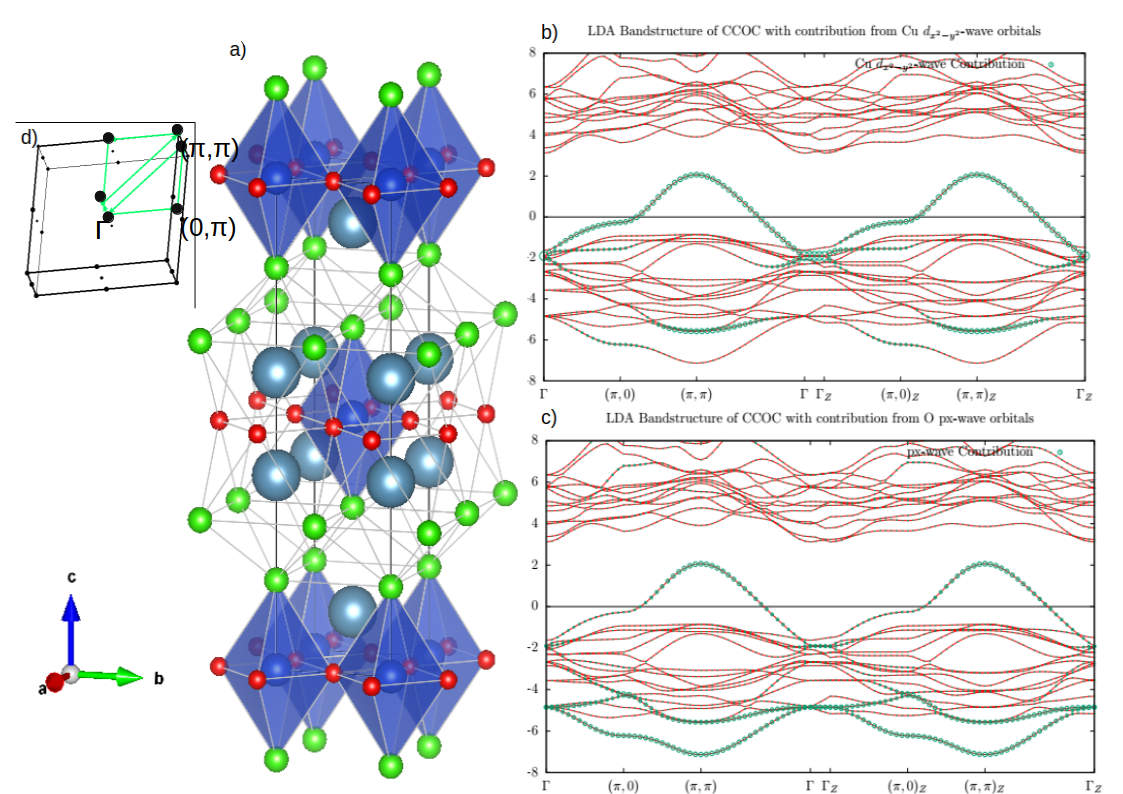
\includegraphics[scale=0.5]{crystal-structure-LDA-CCOC-kpath.png}
    \captionof{figure}{\textbf{a)} CCOC crystal structure. Green balls : Cl, red balls : O, dark blue balls : Cu, light blue balls : Ca. \textbf{b) and c)} Bandstructure of undoped CCOC with contribution from $d_{x^{2}-y^{2}}$ and $p_{x}$ orbitals respectively. \textbf{d)} : k-path used in the Brillouin Zone for the LDA calculation.}
    \label{CCOC-struct}
\end{figure*}
This strong d-wave character of the pseudo-gap motivates the use of theoretical 
tools suited for such correlated orbitals. We chose to work within the framework 
of Dynamical Mean Field Theory \cite{Review-georges} (DMFT) which is known for 
being powerful when dealing with correlated materials. The anti-ferromagnetic 
Mott insulator phase at low doping also motivates the use of DMFT. Indeed, the 
Mott insulator phase is due to two-body interactions which can be captured 
within DMFT, but not within the one-particle picture of Density Functional 
Theory (DFT). Moreover, it has been shown that the investigation of the 
pseudo-gap phase using DMFT requires to take into account non-local correlations 
\cite{huscroft2001pseudogaps,lichtenstein2000antiferromagnetism}. Indeed, as the 
pseudo-gap is an anisotropic feature, and since it is needed to account for the 
anti-ferromagnetic fluctuations, k-dependent observables are needed so the local 
self-energy approximation of single-site DMFT would prevent us to capture the 
PG. Hence we will use an extension of DMFT : Cluster DMFT (C-DMFT) 
\cite{kotlier-CDMFT,maier-cluster-theories} in which the lattice problem is 
mapped onto a cluster of atoms embedded in a self-consistent bath of free 
electrons. This cluster of multiple atoms allows the anti-ferromagnetic 
fluctuations to be included. Such a construction allows us to take into account 
explicitly the correlations inside the cluster, i.e correlations on the size of 
the cluster will be treated exactly. This is more powerful than standard 
single-site DMFT that only considers on-site correlations. In this study, we 
will consider oriented 2-site clusters, which are supposed to be the minimal 
cluster size to investigate the pseudo-gap phase 
\cite{huscroft2001pseudogaps,lichtenstein2000antiferromagnetism}. The similarity 
of the hybridization of d- and p-orbitals in CCOC with the effective single-band 
Zhang-Rice singlet suggest that we can treat the problem within C-DMFT 
considering only one effective band on each atom of the cluster. This effective 
band will be extracted from LDA calculations. The strong 2D character of the 
$\mathrm{CuO_{2}}$ layers allows us to consider a 2D Hubbard Hamiltonian with 
nearest, next-nearest and next-next-nearest neighbor hopping within the 2 
dimensional plane, and on-site interactions between electrons. The layers are so 
well separated that we can neglect the interactions between each other. \par I 
will first review the idea and concepts behind C-DMFT and then its practical 
implementation with oriented 2-sites clusters. I will then compare first 
preliminary results with 'benchmark' results \cite{benchmark2Dcubic} obtained 
with Quantum Monte Carlo  techniques. This comparison is necessary to confirm 
that the program I wrote matches with results that are well established and 
reliable. Then I will present calculations of the electronic structure of CCOC 
using DFT+C-DMFT and the computed optical properties of such compounds.
\end{multicols}
\section{Theory and Implementation of Cluster-Dynamical Mean Field Theory}
\subsection{Single-site Dynamical Mean Field Theory}

\subsection{Towards Dimer Dynamical Mean Field Theory}

\subsection{Analytic continuation}

\subsection{Optical Conductivity}

\section{Results and discussion}
\subsection{Single-site versus dimer Dynamical Mean Field Theory}

\subsection{$\mathrm{Ca_{2}CuO_{2}Cl_{2}}$}

\section{Conclusion}

\begin{multicols}{2}
\bibliographystyle{plain}
\bibliography{references.bib}
\end{multicols}
\end{document}
